\chapter{Resultados e Discussões}
\label{cap:resultados}

% - - - - - - - - - - - - - - - - - - - - - - - - - - - - - - - - - - -------
Neste capítulo serão apresentados os testes no protótipo e a análise dos resultados. Para execução dos testes, foram levadas em consideração algumas possíveis restrições para captura da imagem pelo celular, para que não afete o funcionamento do algoritmo. 

A folha do teste deve estar em uma superfície plana e o celular deve estar posicionado a uma distancia de aproximadamente 30 cm da folha do teste, ele deve ficar paralelo a superfície do teste para uma melhor captura da imagem, deve se respeitar também todas as restrições vistas na Seção 3.3.1. Foram utilizadas no teste as folhas do modelo II conforme seção 2.2.1. Ao todo, foram utilizadas 10 imagem do teste palografico.

Na tabela \ref{tab:result}  temos o resultado da contagem para as imagens utilizadas nos testes. Foi feito uma comparação entre a contagem manual dos palos e a contagem feito pelo protótipo, temos também a quantidades de palos detectados pelo contador que não estão presentes no total real, temos a quantidade de palos não detectados pelo contador e o percentual de acertos pelo protótipo. Foi denominado falso positivo quando o algoritmo detecta palos a mais que a quantidade feita na contagem manual e falso negativo quando alguns palos não são detectados.
No decorrer do experimento, foi observado que esses erros de detecção ocorrem na etapa de segmentação. Os falsos positivos geralmente ocorrem quando o palo esta meio apagado ou quando o palo não tem um tonalidade de cinza constante. Gerando mais objetos que a quantidade real, como pode ser visto na figura \ref{fig:palo-seg}.

\begin{figure}[H]
 \centering
 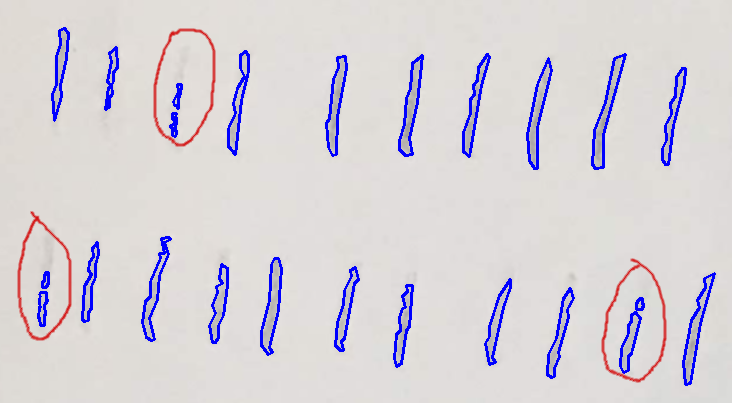
\includegraphics[width=0.50\textwidth]{./fig/resultado-analise/seg-palo}
 \caption{Segmentação de falsos positivos.}
  Fonte: O autor.
 \label{fig:palo-seg}
\end{figure}

Já os falsos negativos ocorrem quando os palos estão muito próximos ou encostado um no outro, dificultando a segmentação fazendo com que dois ou mais palos sejam contados como apenas um. Como pode ser visto na figura \ref{fig:palo-seg}  .

\begin{figure}[H]
 \centering
 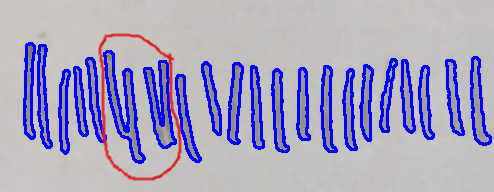
\includegraphics[width=0.50\textwidth]{./fig/resultado-analise/seg-palos}
 \caption{Segmentação de falsos negativos.}
  Fonte: O autor.
 \label{fig:palo-seg}
\end{figure}


\begin{table*}[hp]
\centering
\begin{tabular}{|l|l|l|l|l|l|}
\hline
\textbf{Teste} & \textbf{\begin{tabular}[c]{@{}l@{}}Contagem \\ Manual\end{tabular}} & \textbf{\begin{tabular}[c]{@{}l@{}}Contagem \\ prototipo\end{tabular}} & \textbf{\begin{tabular}[c]{@{}l@{}}Falso \\ positivo\end{tabular}} & \textbf{\begin{tabular}[c]{@{}l@{}}Falso \\ negativo\end{tabular}} & \textbf{\%Acerto} \\ \hlin
1              & 805    & 785       & 0      & 20    & 97,51\%        \\ \hline
2              & 620    & 620       & 0      & 0      & 100\%           \\ \hline
3              & 688    & 684       & 0      & 4      & 99,41\%        \\ \hline
4              & 632    & 633       & 1      & 0      & 99,84\%        \\ \hline
5              & 945    & 945       & 0      & 0      & 100\%           \\ \hline
6              & 577    & 575       & 0      & 2      & 99,65\%        \\ \hline
7              & 856    & 858       & 3      & 1      & 99,53\%        \\ \hline
8              & 818    & 815       & 0      & 3      & 99,75\%        \\ \hline
9              & 907    & 900       & 0      & 7      & 99,22\%        \\ \hline
10            & 1008  & 995       & 0      & 13    & 98,71\%        \\ \hline

\end{tabular}
\caption{Comparação dos resultados da contagem manual com a contagem feito pelo protótipo}
\label{tab:result}
\end{table*}

Somando-se os palos de todos os testes temos 7856 palos, com apenas  54 erros cometidos pelo protótipo, obtendo uma taxa de acerto no geral de 99.31\% o que é um resultado promissor. Podemos notar que a diferença entre os valores reais e os obtidos na contagem é pequena sendo a maior no teste numero 1 com 20 erros. Os melhores resultados foram nos testes numero 2 e 5 contabilizando a quantidade exata dos palos. Nas demais, a menor taxa de acerto foi no teste numero 1, com valor de 97,51\%  de acerto.

O protótipo resultante deste trabalho  mostrou-se promissor, mostrando que o uso de técnicas de processamento de imagens e visão computacional tem se tornando de grande ajuda na resolução de problemas do dia a dia, como podemos ver nos trabalho de \cite{SILVA2012},  que utiliza as mesmas técnicas utilizadas neste trabalho é que também mostra resultados positivos. Ainda que os resultados tenham sido positivos,  se faz necessário mais testes de maneira exaustiva para um melhor grau de acurácia e confiabilidade, porém para o propósito deste trabalho os resultados são satisfatórios.

Uma característica importante neste protótipo é que ele utiliza de imagens obtidas por celular, não há a necessidade de aquirir nenhum equipamento específico para o contagem dos palos, como acontece no software \cite{skip2018}.







